\chapter{Cell Complexes}
\section{Cell Complexes and CW Complexes}
An open $n$-\textbf{cell} is any topological space that is homeomorphic to the open unit ball $\B^n$, and a closed $n$-cell is any space homeomorphic to 
$\widebar{\B}^n$. Every open or closed ball in $\R^n$ is obviously an open or closed cell. The next proposition gives many more examples.
\begin{proposition}\label{CW compact convex is n-cell}
If $D\sub\R^n$ is a compact convex subset with nonempty interior, then $D$ is a closed $n$-cell and its interior is an open $n$-cell. In fact, given any point 
$p\in\Int D$, there exists a homeomorphism $F:\widebar{\B}^n\to D$ that sends $0$ to $p$, $\B^n$ to $\Int D$, and $S^{n-1}$ to $\partial D$.
\end{proposition}
\begin{proof}
Let $p$ be an interior point of $D$. By replacing $D$ with its image under the
translation $x\mapsto x-p$ (which is a homeomorphism of $\R^n$ with itself), we can assume that $p=0\in\Int D$. Then there is some $\eps>0$ such that the ball 
$\B(0,\eps)$ is contained in $D$; using the dilation $x\mapsto x/\eps$, we can assume $\B^n=\B(0,1)\sub D$.\par
The core of the proof is the following claim: \textbf{each closed ray starting at the origin intersects $\partial D$ in exactly one point}. Let $R$ be such a closed 
ray. Because $D$ is compact, its intersection with $R$ is compact; thus there is a point $x_0$ in this intersection at which the distance to the origin assumes its 
maximum. This point is easily seen to lie in the boundary of $D$. To show that there can be only one such point, we show that the line segment from $0$ to $x_0$ 
consists entirely of interior points of $D$, except for $x_0$ itself. Any point on this segment other than $x_0$ can be written in the form $\lambda x_0$ for 
$0\leq\lambda<1$. Suppose $z\in\B(\lambda x_0,1-\lambda)$, and let $y=(z-\lambda x_0)/(1-\lambda)$. A straightforward computation shows that $|y|<1$, so 
$y\in\B(0,1)\sub D$. Since $y$ and $x_0$ are both in $D$ and $z=\lambda x_0+(1-\lambda)y$, it follows from convexity that $z\in D$. Thus the open ball 
$\B(\lambda x_0,(1-\lambda))$ is contained in $D$, which implies that $\lambda x_0$ is an interior point.\par
Now we define a map $f:\partial D\to S^{n-1}$ by
\[f(x)=\dfrac{x}{|x|}.\]
In words, $f(x)$ is the point where the line segment from the origin to $x$ intersects the unit sphere. Since $f$ is the restriction of a continuous map, it is 
continuous, and the discussion in the preceding paragraph shows that it is bijective. Since $\partial D$ is compact, $f$ is a homeomorphism by the closed map lemma.\par
Finally, define $F:\widebar{\B}^n\to D$ by
\[F(x)=\begin{cases}
|x|f^{-1}\Big(\dfrac{x}{|x|}\Big),&x\neq 0;\\
0,&x=0.
\end{cases}\]
Then $F$ is continuous away from the origin because $f^{-1}$ is, and at the origin because boundedness of $f^{-1}$ implies $F(x)\to 0$ as $x\to 0$. Geometrically, $F$ 
maps each radial line segment connecting $0$ with a point $w\in S^{n-1}$ linearly onto the radial segment from $0$ to the point $f^{-1}(w)\in\partial D$. By convexity, 
$F$ takes its values in $D$. The map $F$ is injective, since points on distinct rays are mapped to distinct rays, and each radial segment is mapped linearly to its image. 
It is surjective because each point $y\in D$ is on some ray from $0$. By the closed map lemma, $F$ is a homeomorphism.
\end{proof}
Thus every closed interval in $\R$ is a closed $1$-cell; every compact region in the plane bounded by a regular polygon is a closed $2$-cell; and a solid tetrahedron 
and a solid cube are closed $3$-cells. By our conventions, any singleton is both a closed $0$-cell and an open $0$-cell.
\subsection{Cell Decompositions}
Suppose $X$ is a nonempty topological space, $\{D_\alpha\}_{\alpha\in A}$ is an indexed collection of closed $n$-cells for some fixed $n\geq1$, and for each $\alpha$, 
we are given a continuous map $\varphi_\alpha:\partial D_\alpha\to X$. Letting $\varphi:\amalg_\alpha\partial D_\alpha$ be the map whose restriction to each 
$\partial D_\alpha$ is $\varphi_\alpha$, we can form the adjunction space $X\cup_\varphi(\coprod_\alpha D_\alpha)$. Any space homeomorphic to such an adjunction space 
is said to be obtained from $X$ by attaching $n$-cells to $X$.\par 
For example, $S^2$ can be obtained by attaching a single $2$-cell to $\widebar{\B}^2$. If $Y$ is obtained from $X$ by attaching $n$-cells, then we can view $X$ as a 
closed subspace of $Y$, and as a set, $Y$ is the disjoint union of $X$ and a collection of disjoint open $n$-cells, one for each $\alpha$.\par
If $X$ is a nonempty topological space, a \textbf{cell decomposition} of $X$ is a partition $\mathcal{E}$ of $X$ into subspaces that are \textit{open} cells of various 
dimensions, such that the following condition is satisfied: for each cell $e\in\mathcal{E}$ of dimension $n\geq1$, there exists a continuous map $\varPhi$ from some 
\textit{closed} $n$-cell $D$ into $X$ (called a \textbf{characteristic map} for $e$) that restricts to a homeomomorphism from $\Int D$ onto $e$ and maps $\partial D$ 
into the union of all cells of $\mathcal{E}$ of dimensions strictly less than $n$. A \textbf{cell complex} is a Hausdorff space $X$ together with a specific cell 
decomposition of $X$. (The Hausdorff condition is included both to rule out various pathologies and because, as we show below, the inductive construction of cell 
complexes automatically yields Hausdorff spaces.)\par
A \textbf{finite cell complex} is one whose cell decomposition has only finitely many cells. A cell complex is called \textbf{locally finite} if the collection of 
open cells is locally finite. This is equivalent to the requirement that the collection $\widebar{\mathcal{E}}=\{\widebar{e}:e\in\mathcal{E}\}$ be locally finite.
\subsection{CW Complexes}
Suppose $X$ is a topological space, and $\mathcal{B}$ is any family of subspaces of $X$ whose union is $X$. To say that the topology of $X$ is 
\textbf{coherent with $\mathcal{B}$} means that a subset $U\sub X$ is open in $X$ if and only if its intersection with each $B\in\mathcal{B}$ is open in $B$. It is easy 
to show by taking complements that this is equivalent to the requirement that $U$ is closed in $X$ if and only if $U\cap B$ is closed in $B$ for each $B\in\mathcal{B}$. 
(In either case, the only if implication always holds by definition of the subspace topology on $B$, so it is the if part that is significant.) For example, if 
$(X_\alpha)$ is an indexed family of topological spaces, the disjoint union topology on $\coprod_\alpha X_\alpha$, is coherent with the family $(X_\alpha)$ thought of 
as subspaces of the disjoint union. A space is \textbf{compactly generated} if and only if its topology is coherent with the family consisting of all of its compact 
subsets.\par
The next proposition expresses some basic properties of coherent topologies.
\begin{proposition}\label{coherent topo}
Suppose $X$ is a topological space whose topology is coherent with a family $\mathcal{B}$ of subspaces.
\begin{itemize}
\item[(\rmnum{1})] If $Y$ is another topological space, then a map $f:X\to Y$ is continuous if and only if $f|_B$ is continuous for every $B\in\mathcal{B}$.
\item[(\rmnum{2})] The map $p:\coprod_{B\in\mathcal{B}}B\to X$ induced by inclusion of each set $B\hookrightarrow X$ is a quotient map.
\end{itemize}
\end{proposition}
\begin{proof}
If $f:X\to Y$ is a continuous map, then $f|_B$ is clearly continuous on every $B\in\mathcal{B}$. Conversely, if $f:X\to Y$ is a map such that $f|_B$ is continuous. Let 
$V\sub Y$ be an open set, then for any $B\in\mathcal{B}$ we have
\[f^{-1}(V)\cap B=(f|_B)^{-1}(V).\]
Since $f|_B$ is continuous, the right-hand side is open for every $B\in\mathcal{B}$. Therefore by the coherent condition, $f^{-1}(V)$ is open, and thus $f$ is also 
continuous. This proves (\rmnum{1})\par
For (\rmnum{2}), since $\bigcup B=X$, the map $p$ is surjective. Moreover, let $U$ be a subset of $X$, then
\[p^{-1}(U)=\coprod_{B\in\mathcal{B}}(U\cap B).\]
From the topology on $\coprod_{B\in\mathcal{B}}B$ we know that $p^{-1}(B)$ is open if and only if each $U\cap B$ is open, which by the coherent condition is equivalent 
to $U$ is open. Therefore $p$ is a quotient map.
\end{proof}
A \textbf{CW complex} is cell complex $(X,\mathcal{E})$ satisfying the following additional conditions:
\begin{itemize}
\item[(C)] The closure of each cell is contained in a union of finitely many cells.
\item[(W)] The topology of $X$ is coherent with the family of closed subspaces $\{\widebar{e}:e\in\mathcal{E}\}$.
\end{itemize}
A cell decomposition of a space $X$ satisfying (C) and (W) is called a \textbf{CW decomposition} of $X$. The letters C and W come from the names originally given to 
these two conditions by the inventor of CW complexes, J.H.C. Whitehead: condition (C) was called \textbf{closure finiteness}, and the coherent topology described in 
condition (W) was called the \textbf{weak topology} associated with the subspaces $\{\widebar{e}:e\in\mathcal{E}\}$.\par
For locally finite complexes (and thus all finite ones), conditions (C) and (W) are automatic, as the next proposition shows.
\begin{proposition}\label{CW locally finite cell}
Let $X$ be a Hausdorff space, and let $\mathcal{E}$ be a cell decomposition of $X$. If $\mathcal{E}$ is locally finite, then it is a CW decomposition.
\end{proposition}
\begin{proof}
To prove condition (C), observe that for each $e\in\mathcal{E}$, every point of $\widebar{e}$ has a neighborhood that intersects only finitely many cells of 
$\mathcal{E}$. Because $\widebar{e}$ is compact, it is covered by finitely many such neighborhoods.\par
To prove (W), suppose $A\sub X$ is a subset whose intersection with $\widebar{e}$ is closed in $\widebar{e}$ for each $e\in\mathcal{E}$. Given $x\in X\setminus A$, let 
$W$ be a neighborhood of $x$ that intersects the closures of only finitely many cells, say $\widebar{e}_1,\cdots,\widebar{e}_m$. Since $A\cap\widebar{e}_i$ is closed in 
$\widebar{e}_i$ and thus in $X$, it follows that
\[W\setminus A=W\setminus\big((A\cap\widebar{e}_1)\cap\cdots\cap (A\cap\widebar{e}_m)\big)\]
is a neighborhood of $x$ contained in $X\setminus A$. Thus $X\setminus A$ is open, so $A$ is closed.
\end{proof}
Suppose $X$ is a CW complex. If there is an integer $n$ such that all of the cells of $X$ have dimension at most $n$, then we say $X$ is \textbf{finite-dimensional}; 
otherwise, it is \textbf{infinite-dimensional}. If it is finite-dimensional, the dimension of $X$ is the largest $n$ such that $X$ contains at least one $n$-cell. Of 
course, a finite complex is always finite-dimensional.\par
Here is one situation in which open cells actually are open subsets.
\begin{proposition}\label{CW n-dim n-cell is open}
Suppose $X$ is an $n$-dimensional CW complex. Then every $n$-cell of $X$ is an open subset of $X$.
\end{proposition}
\begin{proof}
Suppose $e_0$ is an $n$-cell of $X$. If $\varPhi:D\to X$ is a characteristic map for $e_0$, then $\varPhi$, considered as a map onto $\widebar{e}_0$, is a quotient map 
by the closed map lemma. Since $\varPhi^{-1}(e_0)=\Int D$ is open in $D$, it follows that $e_0$ is open in $\widebar{e}_0$. On the other hand, if $e$ is any other cell 
of $X$, then $e_0\cap e=\emp$, so $e_0\cap\widebar{e}$ is contained in $\widebar{e}\setminus e$, which in turn is contained in a union of finitely many cells of 
dimension less than $n$. Since $e_0$ has dimension $n$, it follows that $e_0\cap\widebar{e}=\emp$. Thus the intersection of $e_0$ with the closure of every cell is open, 
so $e_0$ is open in $X$ by condition (W).
\end{proof}
A \textbf{subcomplex} of $X$ is a subspace $Y\sub X$ that is a union of cells of $X$, such that if $Y$ contains a cell, it also contains its closure. It follows 
immediately from the definition that the union and the intersection of any collection of subcomplexes are themselves subcomplexes. For each nonnegative integer $n$, we 
define the \textbf{$\bm{n}$-skeleton} of $X$ to be the subspace $X_n\sub X$ consisting of the union of all cells of dimensions less than or equal to $n$; it is an 
$n$-dimensional subcomplex of $X$.
\begin{theorem}
Suppose $X$ is a CW complex and $Y$ is a subcomplex of $X$. Then $Y$ is closed in $X$, and with the subspace topology and the cell decomposition that it
inherits from $X$, it is a CW complex.
\end{theorem}
\begin{proof}
Obviously $Y$ is Hausdorff, and by definition it is the disjoint union of its
cells. Let $e\sub Y$ denote such a cell. Since $\widebar{e}\sub Y$, the finitely many cells of $X$ that have nontrivial intersections with $\widebar{e}$ must also be 
cells of $Y$, so condition (C) is
automatically satisfied by $Y$. In addition, any characteristic map $\varPhi:D\to X$ for $e$ in $X$ also serves as a characteristic map for $e$ in $Y$.\par
To prove that $Y$ satisfies condition (W), suppose $S\sub Y$ is a subset such that $S\cap\widebar{e}$ is closed in $\widebar{e}$ for every cell $e$ contained in $Y$. 
Let $e$ be a cell of $X$ that is not contained in $Y$. We know that $\widebar{e}\setminus e$ is contained in the union of finitely many cells of $X$; some of these, 
say $e_1,\cdots,e_k$, might be contained in $Y$ ( If there is no such cells, then we conclude $S\cap\widebar{e}=\emp$ and the result follows). Then 
$\widebar{e}_1\cup\cdots\cup\widebar{e}_k\sub Y$ and
\[S\cap \widebar{e}=S\cap(\widebar{e}_1\cup\cdots\cup\widebar{e}_k)\cap\widebar{e}=\big((S\cap\widebar{e}_1)\cup\cdots\cup(S\cap\widebar{e}_k)\big)\cap\widebar{e}\]
which is closed in $\widebar{e}$. It follows that $S$ is closed in $X$ and therefore in $Y$.\par
Finally, to show that $Y$ is closed in $X$, just apply the argument in the preceding paragraph with $S=Y$.
\end{proof}
\begin{proposition}
If $X$ is any CW complex, the topology of $X$ is coherent with the collection of subspaces $\{X_n:n\geq 0\}$.
\end{proposition}
\begin{proof}
This is clear, since any cell is contained in some skeleton $X_n$.
\end{proof}
An open cell $e\sub X$ is called a \textbf{regular cell} if it admits a characteristic map that is a homeomorphism onto $\widebar{e}$. For example, 
Proposition~\ref{CW compact convex is n-cell} shows that the interior of a compact convex subset of $\R^n$ (if nonempty) is a regular $n$-cell in $\R^n$. Every $0$-cell 
is a regular cell by convention. For a regular cell, we can always take the inclusion map $\widebar{e}\hookrightarrow X$ as a characteristic map.\par
Note that if we wish to show a certain open cell $e\sub X$ is a regular cell, it is not sufficient to show only that $\widebar{e}$ is a closed cell; it is necessary to 
exhibit a characteristic map that is a homeomorphism onto its image. For example, the set $\B^2\setminus\{(x,0):0<x<1\}$ is an open $2$-cell in $\R^2$ whose closure is 
a closed $2$-cell, but it is not a regular cell because $\widebar{e}\setminus e$ is not homeomorphic to $S^1$. A CW complex is called a \textbf{regular CW complex} or 
\textbf{regular cell complex} if each of its cells is regular, and the closure of each cell is a finite subcomplex.
\begin{example}\label{CW eg}
\mbox{}
\begin{itemize}
\item[$(a)$] A $0$-dimensional CW complex is just a discrete space; it is a finite complex if and only if it is a finite set.
\item[$(b)$] Recall that a bouquet of circles is a wedge sum of the form $S^1\vee\cdots\vee S^1$. Such a wedge sum has a cell decomposition with one $0$-cell (the base 
point), and a $1$-cell for each of the original circles; for the characteristic maps, we can take the compositions
\[\begin{tikzcd}
I\ar[r,"i"]&S^1\ar[r,"\iota_i"]&S^1\amalg\cdots\amalg S^1\ar[r]&S^1\vee\cdots\vee S^1
\end{tikzcd}\]
where $\omega$ is the quotient map and $\iota_j$ is the inclusion of the $j$ th
copy of $S^1$ into the disjoint union.
\item[$(c)$] In general, a CW complex of dimension less than or equal to $1$ is called a \textbf{graph}. Each $0$-cell of the complex is called a vertex, and each 
$1$-cell is called an \textbf{edge}. A graph is said to be \textbf{finite} if its associated CW complex is finite. Graphs have myriad applications in both pure and 
applied mathematics, and are among the most extensively studied objects in the mathematical discipline known as combinatorics.
\item[$(d)$] Let us construct a regular cell decomposition of $S^n$. Note first that $S^0$, being a finite discrete space, is already a regular $0$-dimensional cell 
complex with two cells. Suppose by induction that we have constructed a regular cell decomposition of $S^{n-1}$ with two cells in each dimension $0,\cdots,n-1$. Now 
consider $S^{n-1}$ as a subspace of $S^n$ (the subset where the $x_{n+1}$ coordinate is zero), and note that the open upper and lower hemispheres of $S^n$ are regular 
$n$-cells whose boundaries lie in $S^{n-1}$. The cell decomposition of $S^{n-1}$ together with these new $n$-cells yields a regular cell decomposition of $S^n$ with 
exactly two cells
in each dimension $0$ through $n$. For each $k=0,\cdots,n$, the $k$-skeleton of this complex is $S^k$.
\item[$(e)$] Here is a different cell decomposition of $S^n$, with only one $0$-cell and one $n$-cell and no others. The $0$-cell is the north pole $(0,\cdots,0,1)$, 
and the characteristic map for the $n$-cell is the map $q:\widebar{\B}^n\to S^n$ which collapses $\partial\widebar{\B}^n$ to a single point.
\item[$(f)$] A regular cell decomposition of $\R$ is obtained by defining the $0$-cells to be the integers, and the $1$-cells to be the intervals $(n,n+1)$ for $n\in\Z$, 
with characteristic maps $\varPhi_n:[n,n+1]\to\R$ given by inclusion. Conditions $(C)$ and $(W)$ are automatic because the decomposition is locally finite.
\end{itemize}
\end{example}
Here are two examples of cell decompositions that are not CW decompositions.
\begin{example}
Let $X\sub\R^2$ be the union of the closed line segments from the origin
to $(1,0)$ and to the points $(1,1/n)$ for $n\in\N$, with the subspace topology. Define a cell decomposition of $X$ by declaring the $0$-cells to be $(0,0)$, $(1,0)$, 
and the points $(1,1/n)$, and the $1$-cells to be the line segments minus their endpoints. This is easily seen to be a cell decomposition that satisfies condition $(C)$. 
However, it does not satisfy condition $(W)$, because the set $\{(1/n,1/n^2):n\in\N\}$ has a closed intersection with the closure of each cell, but is not closed in $X$ 
because it has the origin as a limit point.
\end{example}
\[
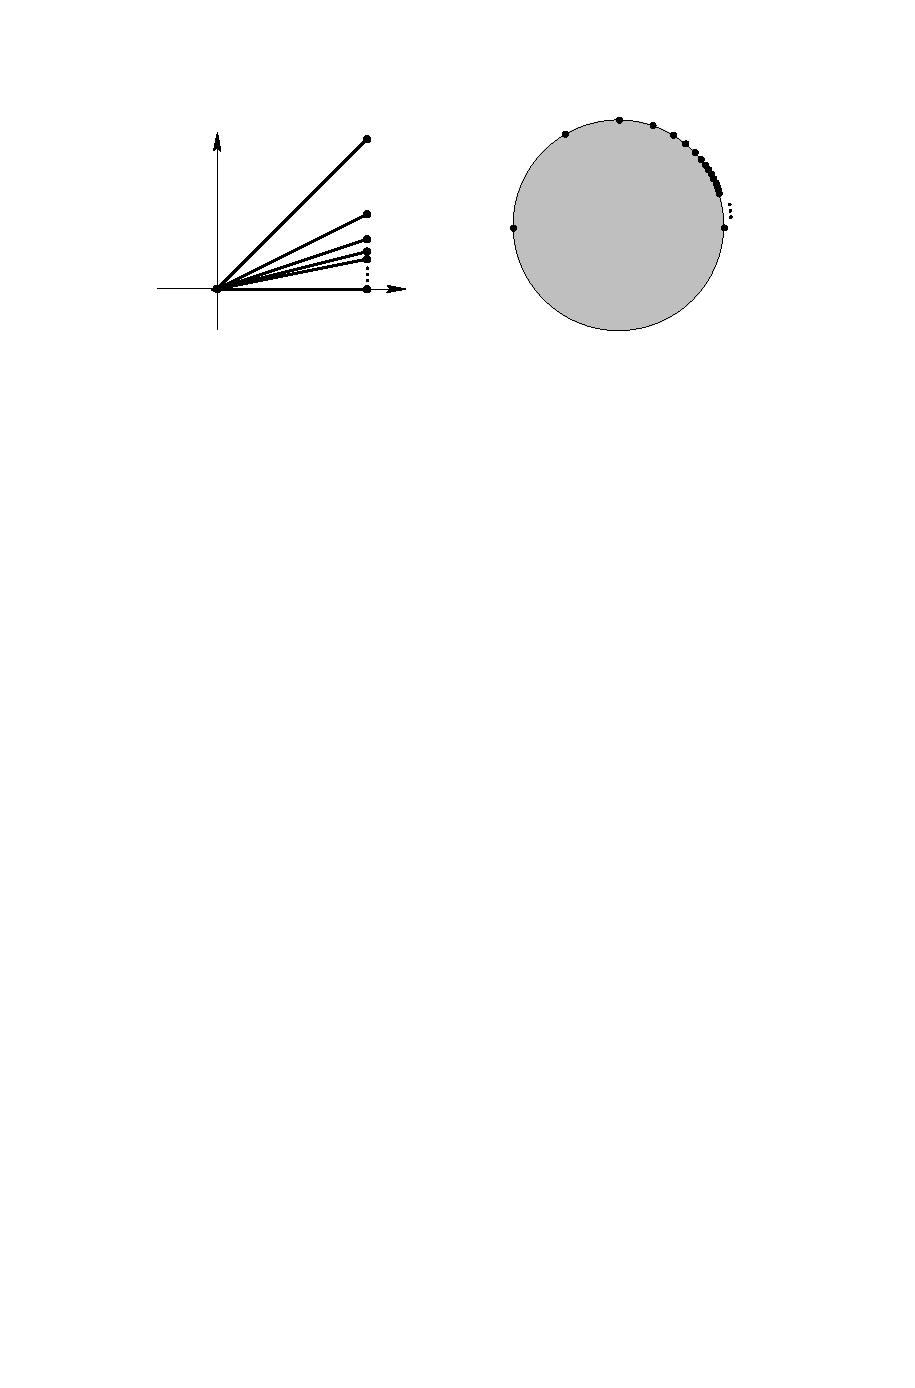
\includegraphics{CWcountereg.pdf}\]
\begin{example}
Define a cell decomposition of $\widebar{\B}^2$ with countably many $0$-cells at the points $\{e^{2\pi i/n}:n\in\N\}$, countably many $1$-cells consisting of the open 
arcs between the $0$-cells, and a single $2$-cell consisting of the interior of the disk. Condition $(W)$ is satisfied for the simple reason that the closure of the 
$2$-cell is $\widebar{\B}^2$ itself, so any set that has a closed intersection with each xe is automatically closed in $\widebar{\B}^2$. But condition $(C)$ does not 
hold.
\end{example}
\section{Topological Properties of CW Complexes}
Many basic topological properties of CW complexes, such as connectedness and compactness, can be read off easily from their CW decompositions.\par
We begin with connectedness. It turns out that this information is already contained in the $1$-skeleton: the next theorem shows, among other things, that a CW complex 
is connected if and only if its $1$-skeleton is connected.
\begin{theorem}\label{CW connected}
For a CW complex $X$, the following are equivalent.
\begin{itemize}
\item[$(a)$] $X$ is path-connected.
\item[$(b)$] $X$ is connected.
\item[$(c)$] The $1$-skeleton of $X$ is connected.
\item[$(d)$] Some $n$-skeleton of $X$ is connected.
\end{itemize}
\end{theorem}
\begin{proof}
Obviously, $(a)\Rightarrow(b)$ and $(c)\Rightarrow(d)$, so it suffices to show that $(b)\Rightarrow(c)$ and $(d)\Rightarrow(a)$.\par
To prove $(b)\Rightarrow(c)$, we prove the contrapositive. Suppose that $X_1=X'_1\cup X''_1$ is a disconnection of the $1$-skeleton of $X$. We show by induction on $n$ 
that for each $n>1$, the $n$-skeleton has a disconnection $X_n=X'_n\cup X''_n$ such that $X'_{n-1}\sub X'_n$ for each $n$. Suppose $X_{n-1}=X'_{n-1}\cup X''_{n-1}$ is 
a disconnection of $X_{n-1}$ for some $n>1$. For each $n$-cell $e$ of $X$, let $\varPhi:D\to X_n$ be a characteristic map. Its restriction to $\partial D$ is a 
continuous map into $X_{n-1}$: since $\partial D= S^{n-1}$ is connected, its image must lie entirely in one of the sets $X'_{n-1}$, $X''_{n-1}$ but not both. Divide 
the $n$-cells into two disjoint collections $\mathcal{E}'$ and $\mathcal{E}''$, according to whether their closures intersect $X'_{n-1}$ or $X''_{n-1}$, respectively, 
and let
\[X'_n=X'_{n-1}\cup\Big(\bigcup_{e\in\mathcal{E}'}e\Big),\quad X''_n=X''_{n-1}\cup\Big(\bigcup_{e\in\mathcal{E}''}e\Big)\]
Clearly $X_n$ is the disjoint union of $X'_n$ and $X''_n$, and both sets are nonempty because $X'_{n-1}$ and $X''_{n-1}$ are nonempty by the inductive hypothesis. If 
$e$ is any cell of $X_n$, its closure is entirely contained in one of these two sets, so $X'_n\setminus\widebar{e}$ is either $\widebar{e}$ or $\emp$, as is $X''_{n}$. 
It follows from condition (W) that both $X'_n$ and $X''_n$ are open (and closed) in $X_n$. This completes the induction.\par
To prove $(d)\Rightarrow(a)$, suppose $X$ is a CW complex whose $n$-skeleton is connected for some $n\geq0$. We show by induction on $k$ that $X_k$ is path-connected 
for each $k\geq n$. It then follows that X is the union of the path-connected subsets $X_k$ for $k\geq n$, all of which have points of $X_n$ in common, so $X$ is 
path-connected.\par
First we need to show that $X_n$ itself is path-connected. If $n=0$, then $X_n$ is discrete and connected, so it is a singleton and thus certainly path-connected. 
Otherwise, choose any point $x_0\in X_n$, and let $S_n$ be the path component of $X_n$ containing $x_0$. For each cell $e$ of $X_n$, note that $\widebar{e}$ is the 
continuous image (under a characteristic map) of a path-connected space, so it is path-connected. Thus if $\widebar{e}$ has a nontrivial intersection with the path 
component $S_n$, it must be contained in $S_n$. It follows that $S_n\cap\widebar{e}$ is closed and open in $\widebar{e}$ for each $e$ (the intersection is either 
$\widebar{e}$ or $\emp$), so $S_n$ is closed and open in $X_n$. Since we are assuming that $X_n$ is connected, it follows that $S_n=X_n$.\par
Now, assume we have shown that $X_{k-1}$ is path-connected for some $k>n$, and
let $S_k$ be the path component of $X_k$ containing $X_{k-1}$. For each $k$-cell e, its closure $\widebar{e}$ is a path-connected subset of $X_k$ that has a nontrivial 
intersection with $X_{k-1}$, so it is contained in $S_k$. It follows that $X_k=S_k$, and the induction is complete.
\end{proof}
Next we address the question of compactness, which is similarly easy to detect
in CW complexes. First we establish two simple preliminary results.
\begin{lemma}\label{CW closure contained finite subcomplex}
In any CW complex, the closure of each cell is contained in a finite subcomplex.
\end{lemma}
\begin{proof}
Let $X$ be a CW complex, and let $e\sub X$ be an $n$-cell; we prove the lemma
by induction on $n$. If $n=0$, then $\widebar{e}=e$ is itself a finite subcomplex, so assume the lemma is true for every cell of dimension less than $n$. Then by 
condition (C), $\widebar{e}\setminus e$ is contained in the union of finitely many cells of lower dimension, each of which is contained in a finite subcomplex by the 
inductive hypothesis. The union of these finite subcomplexes together with $e$ is a finite subcomplex containing $\widebar{e}$.
\end{proof}
\begin{lemma}\label{CW subset discrete iff}
Let $X$ be a CW complex. A subset of $X$ is discrete if and only if its
intersection with each cell is finite.
\end{lemma}
\begin{proof}
Suppose $S\sub X$ is discrete. For each cell $e$ of $X$, the intersection $S\cap\widebar{e}$ is a discrete subset of the compact set $\widebar{e}$, so it is finite, and 
thus so also is $S\cap e$.\par
Conversely, suppose $S$ is a subset whose intersection with each cell is finite. Because the closure of each cell is contained in a finite subcomplex, the hypothesis 
implies that $S\cap\widebar{e}$ is finite for each $e$. This means that $S\cap\widebar{e}$ is closed in $\widebar{e}$, and thus by condition (W), $S$ is closed in $X$. 
But the same argument applies to every subset of $S$; thus every subset of $S$ is closed in $X$, which implies that the subspace topology on $S$ is discrete.
\end{proof}
\begin{theorem}\label{CW subset compact iff}
Let $X$ be a CW complex. A subset of $X$ is compact if and only if it is closed in $X$ and contained in a finite subcomplex.
\end{theorem}
\begin{proof}
Every finite subcomplex $Y\sub X$ is compact, because it is the union of finitely many compact sets of the form $\widebar{e}$. Thus if $K\sub X$ is closed and contained 
in a finite subcomplex, it is also compact.\par
Conversely, suppose $K\sub X$ is compact. If $K$ intersects infinitely many cells, by choosing one point of $K$ in each such cell we obtain an infinite discrete subset 
of $K$, which is impossible. Therefore, $K$ is contained in the union of finitely many cells, and thus in a finite subcomplex by 
Lemma~\ref{CW closure contained finite subcomplex}.
\end{proof}
\begin{corollary}\label{CW compact iff}
A CW complex is compact if and only if it is a finite complex.
\end{corollary}
\begin{proposition}\label{CW locally compact iff}
A CW complex is locally compact if and only if it is locally finite.
\end{proposition}
\begin{proposition}\label{CW maps are char map iff}
Given a Hausdorff space $X$ and a family of maps $\varPhi_\alpha:D^n_\alpha\to X$, then these maps are the characteristic maps of a CW complex structure on $X$ iff:
\begin{itemize}
\item[(\rmnum{1})]Each $\varPhi_\alpha$ restricts to a homeomorphism from $\Int D^n_\alpha$ onto its image, a cell $e^n_\alpha\sub X$, and these cells are all disjoint 
and their union is $X$.
\item[(\rmnum{2})]For each cell $e^n_\alpha$, $\varPhi_\alpha(\partial D^n_\alpha)$ is contained in the union of a finite number of cells of dimension less than $n$.
\item[(\rmnum{3})]A subset of $X$ is closed iff it meets the closure of each cell of $X$ in a closed set.
\end{itemize}
\end{proposition}
Condition (\rmnum{3}) can be restated as saying that a set $C\sub X$ is closed iff $\varPhi^{-1}_\alpha(C)$ is closed in $D^n_\alpha$ for all $\alpha$, since a map from 
a compact space onto a Hausdorff space is a quotient map. In particular, if there are only finitely many cells then (\rmnum{3}) is automatic since in this case the 
projection $\coprod_\alpha D^n_\alpha\to X$ is a map from a compact space onto a Hausdorff space, hence is a quotient map.\par
For an example where all the conditions except the finiteness hypothesis in (\rmnum{2}) are satisfied, take $X$ to be $D^2$ with its interior as a $2$ cell and each 
point of $\partial D^2$ as a $0$ cell. The identity map of $D^2$ serves as the $\varPhi_\alpha$ for the $2$ cell. Condition (\rmnum{3}) is satisfied since it is a 
nontrivial condition only for the $2$ cell.
\begin{proof}
We have already taken care of the only if implication. For the converse, suppose inductively that $X_{n-1}$, the union of all cells of dimension less than $n$, is a CW complex with the appropriate $\varPhi_\alpha$'s as characteristicmaps. The induction can start with $X_{-1}=\emp$. Let $f:X_{n-1}\coprod_\alpha D^n_\alpha\to X_n$ be given by the inclusion on $X_{n-1}$ and the maps $\varPhi_\alpha$ for all the $n$ cells of $X$. This is a continuous surjection, and if we can show it is a quotient map, then $X_n$ will be obtained from $X_{n-1}$ by attaching the $n$ cells $e^n_\alpha$. Thus if $C\sub X_n$ is such that $f^{-1}(C)$ is closed, we need to show that $C\cap\widebar{e}^m_\beta$ is closed for all cells $e^m_\beta$ of $X$, the bar denoting closure.\par
There are three cases. If $m<n$ then $f^{-1}(C)$ closed implies $C\cap X_{n-1}$ closed, hence $C\cap\widebar{e}^m_\beta$ is closed since $\widebar{e}^m_\beta\sub X_{n-1}$. If $m=n$ then $e^m_\beta$ is one of the cells $e^n_\alpha$, so $f^{-1}(C)$ closed implies $f^{-1}(C)\cap D^n_\alpha$ is closed, hence compact, hence its image $C\cap\widebar{e}^n_\alpha$ under $f$ is compact and therefore closed. Finally there is the case $m>n$. Then $C\sub X_n$ implies $C\cap\widebar{e}^m_\beta\sub\varPhi_\beta(\partial D^m_\beta)$. The latter space is contained in a finite union of $\widebar{e}^\ell_\gamma$'s with $\ell<m$. By induction on $m$, each $C\cap\widebar{e}^\ell_\beta$ is closed. Hence the intersection of $C$ with the union of the finite collection of $\widebar{e}^\ell_\gamma$'s is closed. Intersecting this closed set with $\widebar{e}^m_\beta$, we conclude that $C\cap\widebar{e}^m_\beta$ is closed.\par
It remains only to check that $X$ has the weak topology with respect to the $X_n$'s, that is, a set in $X$ is closed iff it intersects each $X_n$ in a closed set. The preceding argument with $C=X_n$ shows that $X_n$ is closed, so a closed set intersects each $X_n$ in a closed set. Conversely, if a set $C$ intersects $X_n$ in a closed set, then $C$ intersects each $\widebar{e}^n_\alpha$ in a closed set, so $C$ is closed in $X$ by (\rmnum{3}).
\end{proof}
\section{Inductive Construction of CW Complexes}
\begin{lemma}\label{char quotient map}
Suppose $X$ is a CW complex, $\{e_\alpha\}_{\alpha\in A}$ is the collection of cells of $X$, and for each $\alpha\in A$, $\varPhi_\alpha:D_\alpha\to X$ is a characteristic map for the cell $e_\alpha$. Then the map $\varPhi:\coprod_\alpha D_\alpha\to X$ whose restriction to each $D_\alpha$ is $\varPhi_\alpha$ is a quotient map.
\end{lemma}
\begin{proof}
The map $\varPhi$ can be expressed as the composition of two maps: the map $\varPhi_1:\coprod_\alpha D_\alpha\to \coprod_\alpha \widebar{e}_\alpha$ whose restriction to each $D_\alpha$ is $\varPhi_\alpha:D_\alpha\to\widebar{e}_\alpha$ followed by the map $\varPhi_2:\coprod_\alpha\widebar{e}_\alpha\to X$ induced by inclusion of each set $\widebar{e}_\alpha$. The first is a quotient map by the closed map lemma, and the second by Proposition~\ref{coherent topo}.
\end{proof}
\begin{proposition}\label{CW structure by X_n}
Let $X$ be a CW complex. Each skeleton $X_n$ is obtained from $X_{n-1}$ by attaching a collection of $n$-cells.
\end{proposition}
\begin{proof}
Let $\{e^n_\alpha\}$ be the collection of $n$-cells of $X$, and for each $n$-cell $e^n_\alpha$, let $\varPhi_\alpha^n:e^n_\alpha\to X$ be a characteristic map. Define $\varphi:\coprod_\alpha\partial D^n_\alpha\to X$ to be the map
whose restriction to each $\partial D^n_\alpha$ is equal to the restriction of $\varPhi^n_\alpha$. By definition of a cell complex, $\varphi$ takes its values in $X_{n-1}$, so we can form the adjunction space $X_{n-1}\cup_\varphi(\coprod_\alpha D^n_\alpha)$.\par
The map $\varPhi:X_{n-1}\amalg(\coprod_\alpha D_\alpha^n)\to X_n$ that is equal to inclusion on $X_{n-1}$ and to $\varPhi^n_\alpha$ on each $D^n_\alpha$ makes the same identifications as the quotient map defining the adjunction space, so if we can show that $\varPhi$ is a quotient map, then uniqueness of quotient spaces shows that $X_n$ is homeomorphic to the adjunction space described
in the preceding paragraph.\par
Suppose therefore that $A$ is a saturated closed subset of the disjoint union, and let $B=\varPhi(A)$, so that $A=\varPhi^{-1}(B)$. The hypothesis means that $A\cap X_{n-1}$ is closed in $X_{n-1}$ and $A\cap D_\alpha^n$ is closed in $D_\alpha^n$ for each $\alpha$. The first assertion implies that $B\cap\widebar{e}$ is closed in $\widebar{e}$ for every cell $e$ of dimension less than $n$; and the second implies that $B\cap \widebar{e^n_\alpha}$ is closed in $\widebar{e^n_\alpha}$ for each $n$-cell because $\varPhi^n_\alpha:D^n_\alpha\to \widebar{e^n_\alpha}$ is a closed map by the
closed map lemma. Thus $B$ is closed in $X_n$. It follows from the definition that $\varPhi$ is a quotient map.
\end{proof}
The next theorem, which is a sort of converse to Proposition~\ref{CW structure by X_n}, shows how to construct CW complexes by inductively attaching cells.
\begin{theorem}[\textbf{CW Construction Theorem}]\label{CW construction}
Suppose $X_0\sub X_1\sub\cdots\sub X_{n-1}\sub X_n\sub\dots$ is a sequence of topological spaces satisfying the following conditions:
\begin{itemize}
\item[(\rmnum{1})] $X_0$ is a nonempty discrete space.
\item[(\rmnum{2})] For each $n\geq1$, $X_n$ is obtained from $X_{n-1}$ by attaching a (possibly empty) collection of $n$-cells.
\end{itemize}
Then $X=\bigcup_nX_n$ has a unique topology coherent with the family $\{X_n\}$, and a unique cell decomposition making it into a CW complex whose $n$-skeleton is $X_n$ for each $n$.
\end{theorem}
\begin{proof}
Give $X$ a topology by declaring a subset $B\sub X$ to be closed if and only if
$B\cap X_n$ is closed in $X_n$ for each $n$. It is immediate that this is a topology, and it is obviously the unique topology coherent with $\{X_n\}$.With this topology, each $X_n$ is a subspace of $X$: if $B$ is closed in $X$, then $B\cap X_n$ is closed in $X_n$ by definition. Conversely, if $B$ is closed in $X_n$, then by virtue of the fact that each $X_{m-1}$ is closed in $X_m$ by, it follows that $B\cap X_m$ is closed in $X_m$ for each $m$ and thus $B$ is also closed in $X$.\par
Next we define the cell decomposition of $X$. The $0$-cells are just the points of the discrete space $X_0$. For each $n\geq 1$, let
\[q_n:X_{n-1}\amalg\Big(\coprod_{\alpha\in A_n}D^n_\alpha\Big)\to X_n\]
be a quotient map realizing $X_n$ as an adjunction space. It follows that
$X_n\setminus X_{n-1}$ is an open subset of $X_n$ homeomorphic to $\coprod_\alpha\Int D_\alpha^n$, which is a disjoint union of open $n$-cells, so we can define the $n$-cells of $X$ to be the components $\{e^n_\alpha\}$
of $X_n\setminus X_{n-1}$. These are subspaces of $X_n$ and hence of $X$, and $X$ is the disjoint union of all of its cells.\par
For each $n$-cell $e^n_\beta$, define a characteristic map $\varPhi^n_\beta:D^n_\beta\to X$ as the composition
\[\begin{tikzcd}
D^n_\beta\ar[r,hook]&X_{n-1}\amalg\Big(\coprod\limits_{\alpha\in A_n}D^n_\alpha\Big)\ar[r,"q_n"]&X_n\ar[r,hook]&X
\end{tikzcd}\]
Clearly $\varPhi^n_\beta$ maps $\partial D^n_\beta$ into $X_{n-1}$, and its restriction to $\Int D^n_\beta$ is a bijective continuous map onto $e^n_\beta$, so we need only show that this restriction is a homeomorphism
onto its image. This follows because is equal to the inclusion of $\Int D^n_\beta$ into the disjoint union, followed by the restriction of $q_n$ to the saturated open subset $\Int D^n_\beta$, which is a bijective quotient map onto $e^n_\beta$. This proves that $X$ has a cell decomposition for which $X_n$ is the $n$-skeleton for each $n$. Because the $n$-cells of any such decomposition are the components of $X_n\setminus X_{n-1}$ this is the unique such cell decomposition.\par
Next we have to show that $X$ is Hausdorff. It suffices to show that for each $p\in X$, there exists a continuous function $f:X\to[0,1]$ such that $f^{-1}(0)=\{p\}$. To prove the existence of such an $f$ , let $p\in X$ be arbitrary, and let $e^m_{\alpha_0}$ be the unique cell containing $p$, with $m$ the dimension of $e^m_{\alpha_0}$. Let $\varPhi^m_{\alpha_0}:D^m_{\alpha_0}\to X$ be the corresponding characteristic map. We start by defining a map $f_m:X_m\to[0,1]$ as follows. If $m=0$, just let $f_m(p)=0$ and $f_m(x)=1$ for $x\neq p$. Otherwise, let $\widetilde{p}=(\varPhi^m_{\alpha_0})^{-1}(p)\in\Int D^m_{\alpha_0}$. By the result of Exercise~\ref{closed cell exercise}$(a)$, there is a continuous function $F:D^m_{\alpha_0}\to[0,1]$ that is equal to $1$ on $\partial D^m_{\alpha_0}$ and is equal to $0$ exactly at $\widetilde{p}$. Define a function
\[\widetilde{f}_m:X_{m-1}\amalg\Big(\coprod_{\alpha\in A}D^m_\alpha\Big)\to\R\]
by letting $\widetilde{f}_m=F$ on $D^m_{\alpha_0}$ and $\widetilde{f}_m\equiv1$ everywhere else. Then $\widetilde{f}_m$ is continuous
by the characteristic property of the disjoint union, and descends to the quotient to yield a continuous function $f_m:X_m\to[0,1]$ whose zero set is $\{p\}$.\par
Now suppose by induction that for some $n>m$ we have defined a continuous function $f_{n-1}:X_{n-1}\to[0,1]$ such that $f^{-1}_{n-1}(0)=\{p\}$. Define a map $\widetilde{f}_n:X_{n-1}\amalg(\coprod_\alpha D_\alpha^n)\to[0,1]$ as follows. On $X_{n-1}$, we just let $\widetilde{f}_n=f_{n-1}$. Exercise~\ref{closed cell exercise}$(b)$ shows that for each closed $n$-cell $D^n_\alpha$, the function $f_{n-1}\circ\varPhi^n_\alpha|_{\partial D^n_\alpha}:\partial D^n_\alpha\to[0,1]$ extends to a continuous function $F_\alpha^n:D^n_\alpha\to[0,1]$ that has no zeros in $\Int D^n_\alpha$. If we define
\[\widetilde{f}_n:X_{n-1}\amalg\Big(\coprod_{\alpha\in A}D^n_\alpha\Big)\to\R\]
by letting $\widetilde{f}_n=f_{n-1}$ on $X_{n-1}$ and $\widetilde{f}_n=F^n_\alpha$ on $D^n_\alpha$, then as before, $\widetilde{f}_n$ is continuous and descends to the quotient to yield a function $f_n:X_n\to[0,1]$ whose zero set is $\{p\}$.\par
Finally, we just define $f:X\to[0,1]$ by letting $f(x)=f_n(x)$ if $x\in X_n$; our construction ensures that this is well defined, and it is continuous by Proposition~\ref{coherent topo}. This completes the proof that $X$ is Hausdorff, so it is a cell complex.\par
If $X$ contains only finitely many cells, we can stop here, because every finite cell complex is automatically a CW complex. For the general case, we have to prove that $X$ satisfies conditions (C) and (W). First, we prove by induction on $n$ that these conditions are satisfied by $X_n$ for each $n$. They certainly hold for $X_0$ because it is a discrete space. Suppose they hold for $X_{n-1}$, so that $X_{n-1}$ is a CW complex. To prove that $X_n$ satisfies condition (C), just note that for any $k$-cell with $1\leq k\leq n$, $\varPhi^k_\alpha(\partial D^k_\alpha)$ is a compact subset of the CW complex $X_{k-1}$, and therefore by Theorem~\ref{CW subset compact iff} it is contained in a finite subcomplex of $X_{k-1}$. To prove condition (W), suppose $B\sub X_n$ has a closed intersection with $\widebar{e}$ for every cell $e$ in $X_n$. Then $B\cap X_{n-1}$ is closed in $X_{n-1}$ because $X_{n-1}$ satisfies condition (W), and $B\cap\widebar{e^n_\alpha}$ is closed in $\widebar{e^n_\alpha}$ for
every $n$-cell $e^n_\alpha$ by assumption. It follows that $q^{-1}_n(B)$ is closed in $X_{n-1}\amalg(\coprod_\alpha D^n_\alpha)$, so $B$ is closed in $X_n$ by definition of the quotient topology.\par
Finally, we just need to show that $X$ itself satisfies conditions (C) and (W). Condition (C) follows from the argument in the preceding paragraph, because the closure of each cell lies in some $X_n$. To prove (W), suppose $B\sub X$ has a closed intersection with $\widebar{e}$ for every cell $e$ in $X$. Then by the discussion above, $B\cap X_n$ is closed in $X_n$ for each $n$, and therefore $B$ is closed in $X$ by definition of the topology on $X$.
\end{proof}
Here is an interesting example of a CW complex constructed in this way.
\begin{example}
In Example~\ref{CW eg}, we showed how to obtain $S^n$ from $S^{n-1}$ by attaching two $n$-cells. Continuing this process by induction, we obtain an infinite dimensional CW complex $S^\infty=\bigcup_nS^n$ with two cells in every dimension. It contains every $S^n$ as a subcomplex.
\end{example}
The inductive description of CW complexes is often useful in defining maps out
of CW complexes inductively cell by cell. One example of such a construction was the construction of the function $f$ in the proof of Theorem~\ref{CW construction} used to show that $X$ is Hausdorff. The proof of the next theorem uses another example of this technique.
\begin{theorem}\label{CW is paracompact}
Every CW complex is paracompact
\end{theorem}
\begin{proof}
Suppose $X$ is a CW complex, and $\mathcal{U}=(U_\alpha)_{\alpha\in A}$ is an indexed open cover of $X$. We will show that there is a partition of unity $(\psi_\alpha)_{\alpha\in A}$ subordinate to $\mathcal{U}$, it follows that $X$ is paracompact.\par
For each $n$, define $U^n_\alpha:=U_\alpha\cap X_n$. We begin by constructing by induction, for each $n$, a partition of unity subordinate to $(U_\alpha^n)$.\par
For $n=0$, we simply choose for each $x\in X_0$ an $\alpha$ such that $x\in U_\alpha$, and let $\psi^0_\alpha(x)=1$ and $\psi^0_{\alpha'}(x)=0$ for $\alpha'\neq\alpha$.\par
Now suppose that for $k=0,\cdots,n$ we have defined partitions of unity $(\psi^k_\alpha)$ for $X_k$ subordinate to $(U^k_\alpha)$, satisfying the following properties for each $\alpha\in A$ and each $k$:
\begin{itemize}
\item[$(1)$]$\psi^k_\alpha|_{X_{k-1}}=\psi^{k-1}_\alpha$.
\item[$(2)$]If $\psi_\alpha^{k-1}\equiv 0$ on an open subset $V\sub X_{k-1}$, then there is an open subset $V'\sub X_k$ containing $V$ on which $\psi^k_\alpha\equiv0$.
\end{itemize}
Let $q:X_n\amalg(\coprod_{\gamma\in\Gamma}D^{n+1}_\gamma)\to X_{n+1}$ be a quotient map realizing $X_{n+1}$ as an adjunction space obtained by attaching $(n+1)$-cells to $X_n$. We will extend each function $\psi^n_\alpha$ to $X_{n+1}$ cell by cell.\par
Fix $\gamma\in\Gamma$. Let $\varPhi_\gamma:D^{n+1}_\gamma\to X_{n+1}$ be the characteristic map $\varPhi_\gamma:=q|_{D^{n+1}_\gamma}$, and let $\varphi_\gamma=\varPhi_\gamma|_{\partial D^{n+1}_\gamma}:\partial D^{n+1}_\gamma\to X_n$ be the corresponding attaching map. For each $\alpha\in A$, let $\widetilde{\psi}^n_\alpha=\psi^n_\alpha\circ\varphi_\gamma:\partial D^{n+1}_\gamma\to[0,1]$ and $\widetilde{U}^{n+1}_\alpha=\varPhi_\gamma^{-1}(U_\alpha^{n+1})\sub D^{n+1}_\gamma$.\par
For any subset $A\sub\partial D^{n+1}_\gamma$ and $0<\eps<1$, let $A(\varphi)\sub D^{n+1}_\gamma$ be the subset
\[A(\eps)=\{x\in D^{n+1}_\gamma:x/|x|\in A\text{ and }1-\eps<|x|\leq 1\},\]
where the norm $|x|$ is defined with respect to some homeomorphism of $D^{n+1}_\gamma$ with $\widebar{\B}^{n+1}$. In particular, $\partial D_\gamma^{n+1}(\eps)$ is the set of all $x\in D_{\gamma}^{n+1}$ such that $|x|>1-\eps$.\par
By compactness of the set $\varPhi_\gamma(\partial_\gamma^{n+1})$ and local finiteness of the indexed cover $(\supp\psi^n_\alpha)$, there are only finitely many indices  $\alpha$ for which $\widetilde{\psi}_{\alpha_i}^n$ is not identically zero on $\partial D_\gamma^{n+1}$. For each such index, $A_i:=\supp\widetilde{\psi}_{\alpha_i}^n$ is a compact subset
of $\widetilde{U}_{\alpha}^{n+1}\cap\partial D^{n+1}_\gamma$, so there is some $\eps_i\in(0,1)$ such that $A_i(\eps_i)\sub\widetilde{U}^{n+1}_\alpha$. Let $\eps$ be the minimum of $\eps_1,\cdots,\eps_k$, and let $\sigma:D^{n+1}_\gamma\to[0,1]$ be a bump function that is equal to $1$ on $D_\gamma^{n+1}\setminus\partial D^{n+1}_\gamma(\varphi)$ and supported in $\partial D^{n+1}_\gamma(\eps/2)$. Choose a partition of unity $(\eta_\alpha)$ for $D_\gamma^{n+1}$ subordinate to the cover $(\widetilde{U}^{n+1}_\alpha)$, and for each $\alpha\in A$ define $\widetilde{\psi}_\alpha^{n+1}:D_\gamma^{n+1}\to[0,1]$ by
\[\widetilde{\psi}^{n+1}_\alpha(x)=\sigma(x)\eta_\alpha(x)+(1-\sigma(x))\widetilde{\psi}_\alpha^n\Big(\dfrac{x}{|x|}\Big)\]
Then $\widetilde{\psi}_\alpha^{n+1}$ is continuous and supported in $\widetilde{U}_\alpha^{n+1}$ and the restriction of $\widetilde{\psi}_\alpha^{n+1}$ to $\partial D_\gamma^{n+1}$ is equal to $\widetilde{\psi}_\alpha^{n}$. A computation shows that $\sum_\alpha\widetilde{\psi}_\alpha^{n+1}\equiv 1$.\par
Now repeat this construction for each $(n+1)$-cell $D_\gamma^{n+1}$. By construction, $\widetilde{\psi}_\alpha^{n+1}$ passes to the quotient and determines a continuous function $\psi_\alpha^{n+1}\to[0,1]$ supported in $U_\alpha^{n+1}$ and satisfying $(1)$. To check that $(2)$ is also satisfied, suppose $V$ is an open subset of $X_n$ on which $\psi_\alpha^n\equiv 0$. Then for each $\gamma$, there is an open subset $\widetilde{V}(\eps/2)\sub D_\gamma^{n+1}$ on which $\widetilde{\psi}_\alpha^{n+1}\equiv0$ by construction (where $\widetilde{V}=\varphi^{-1}_\gamma(V)$, and $\eps$ may vary with $\gamma$). The union of $V$ together with the images of these sets is an open subset $V'\sub X_{n+1}$ on which $\psi_\alpha^{n+1}\equiv0$. To show that the indexed cover $\supp\psi^{n+1}_\alpha$ is locally finite, let $x\in X_{n+1}$ be arbitrary. If $x$ is in the interior of an $(n+1)$-cell, then that cell is a neighborhood of $x$ on which only finitely many of the functions $\psi_\alpha^{n+1}$ are nonzero by construction. On the other hand, if $x\in X_n$, because $(\psi_\alpha^n)$ is a partition of unity there is some neighborhood $V$ of $x$ in $X_n$ on which $\psi^n_\alpha\equiv0$ except when $\alpha$ is one of finitely many indices, and then $(2)$ shows that $\psi_\alpha^{n+1}\equiv0$ on $V'$ except when $\alpha$ is one of the same indices. Thus $(\psi_\alpha^{n+1})$ forms a partition of unity for $X_{n+1}$ subordinate to $(U_\alpha^{n+1})$. This completes the induction.\par
Finally, for each $\alpha$, define $\psi_\alpha:X\to[0,1]$ to be the function whose restriction to each $X_n$ is equal to $\psi_\alpha^n$. By $(1)$, this is well defined, and because the topology of $X$ is coherent with its $n$-skeleta, it is continuous. Because $\sum_\alpha\psi_\alpha^n\equiv1$ for each $n$, it follows that $\sum_\alpha\psi_\alpha\equiv 1$ on $X$. To prove local finiteness, let $x\in X$ be arbitrary. Then $x\in X_n$ for some $n$, and because $(\psi_\alpha^n)$ is a partition of unity there is some neighborhood $V_n$ of $x$ in $X_n$ on which $\psi_\alpha^n\equiv0$ except for finitely many choices of $\alpha$. Property $(2)$ guarantees that there is a sequence of sets $V_n\sub V_{n+1}\sub\cdots$ on which $\psi_\alpha\equiv0$ except when $\alpha$ is one of the same indices, with $V_k$ open in $X_k$ for each $k$. It
follows that $\bigcup_kV_k$ is a neighborhood of $x$ in $X$ on which all but finitely many of the functions $\psi_\alpha$ are identically zero. Thus $(\psi_\alpha)$ is the required partition of unity.
\end{proof}
\section{CW Complexes as Manifolds}
It is usually relatively easy to show that a CW complex is a manifold
\begin{proposition}\label{CW comp into mani}
Suppose $X$ is a CW complex with countably many cells. If $X$ is locally Euclidean, then it is a manifold.
\end{proposition}
\begin{proof}
Every CW complex is Hausdorff by definition. Lemma~\ref{char quotient map} shows that $X$ is a quotient of a disjoint union of countably many closed cells of various dimensions. Such a disjoint union is easily seen to be second countable, and then by Proposition~\ref{quotient of C2} $X$ is also second countable.
\end{proof}
\begin{proposition}\label{CW dim mani dim}
If $M$ is a nonempty $n$-manifold and a CW complex, then the dimension of $M$ as a CW complex is also $n$.
\end{proposition}
\begin{proof}
For this proof, we assume the theorem on invariance of dimension, that is, the dimension of a manifold is unique. Let $M$ be an $n$-manifold with a given CW decomposition. Because every manifold is locally compact, the CW decomposition is locally finite by Proposition~\ref{CW locally compact iff}. Let $x\in M$ be arbitrary. Then $x$ has a neighborhoodW that intersects the closures of only finitely many cells. Suppose $k$ is the maximum dimension of such cells, and let $e$ be an open $k$-cell of maximum dimension $k$ such that $\widebar{e}_0$ has a nontrivial intersection with $W$. Because $W$ is open, it must contain a point of $e_0$ as well. Let $U=W\cap e_0$. Then $U$ is open in $e_0$, so it is a $k$-manifold. We will show below, using an adaptation of the argument of Proposition~\ref{CW n-dim n-cell is open}, that $U$ is open in $M$, from which it follows that it is also an $n$-manifold, so $k=n$. Since this shows that every point has a neighborhood that intersects no cell of dimension larger than $n$, this completes the proof.\par
To show that $U$ is open, we show that $U\cap\widebar{e}$ is open in $\widebar{e}$ for every cell $e$. It suffices to consider only cells whose closures have nontrivial intersections with $W$. Note that $U\cap e_0=W\cap e_0$ is open in $e_0$ and hence in $\widebar{e}_0$ (since $e_0$ is open in $\widebar{e}_0$). On the other hand, if $e$ is any other open cell whose closure intersects $W$, then $U$ is disjoint from $e$ (because the open cells are disjoint), and $\widebar{e}\setminus e$ is contained in a union of cells of dimension less than $k$, so $U\cap\widebar{e}=\emp$. It follows that $U$ is open in $M$, which completes the proof.
\end{proof}
\section{Classification of 1-Dimensional Manifolds}
In this section, we use the theory of CW complexes to provide a complete classification of connected $1$-manifolds with and without boundary.\par
As a first step toward the classification theorem, we show that every $1$-manifold can be realized as a regular CW complex.
\begin{theorem}
Every $1$-manifold admits a regular CW decomposition
\end{theorem}
\begin{proof}
Let $M$ be a $1$-manifold. By Proposition~\ref{mani regular ball cover} $M$ has a countable cover $\{U_i\}$ by regular coordinate balls. Each such set $U_i$ is a regular $1$-cell and an open subset
of $M$, and its boundary consists of exactly two points. For each $n\in\N$, let $M_n=\widebar{U}_1\cup\cdots\cup\widebar{U}_n$, so $\bigcup_nM_n=M$.\par
To construct a CW decomposition of $M$, we construct a finite regular cell decomposition $\mathcal{E}_n$ of each subset $M_n$ in such a way that $M_{n-1}$ is a subcomplex of $M_n$. Begin by letting $\mathcal{E}_1$ be the collection consisting of the open $1$-cell $U_1$ and its two boundary points. This is a regular cell decomposition of $M_1$.\par
Now let $n\geq1$, and suppose by induction that for each $i=1,\cdots,n$ we have
defined a finite regular cell decomposition $E_i$ of $M_i$ such that $M_{i-1}$ is a subcomplex of $M_i$. For the inductive step, we proceed as follows. Consider the next regular coordinate ball $U_{n+1}$. Some of the finitely many $0$-cells of $\mathcal{E}_n$ might lie in $U_{n+1}$. We obtain a finite regular cell decomposition $\mathcal{C}$ of $\widebar{U}_{n+1}\approx[0,1]$ by letting the $0$-cells of $\mathcal{C}$ be those $0$-cells of $\mathcal{E}_n$ that lie in $U_{n+1}$ together with the two boundary points of $\widebar{U}_{n+1}$, and letting the $1$-cells be the intervening open intervals.\par
We will prove that each of the cells of $\mathcal{C}$ either is contained in a cell of $\mathcal{E}_n$, or is disjoint from all the cells of $\mathcal{E}_n$. This is obvious for the $0$-cells. Consider a $1$-cell $c\in\mathcal{C}$. By construction, $c$ intersects none of the $0$-cells in $\mathcal{E}_n$. Suppose there is some $1$-cell $e\in\mathcal{E}_n$ such that $c\cap e=\emp$. Since $c$ contains no $0$-cells and thus no boundary points of $e$, we have $c\cap e=c\cap\widebar{e}$. Since $e$ is open in $M$ and $\widebar{e}$ is closed in $M$, it follows that $c\cap e$ is both open and closed in $c$. Since $c$ is an open $1$-cell, it is connected, so it follows that $c=c\cap e$, which means $c\sub e$.\par
\begin{figure}
\centering
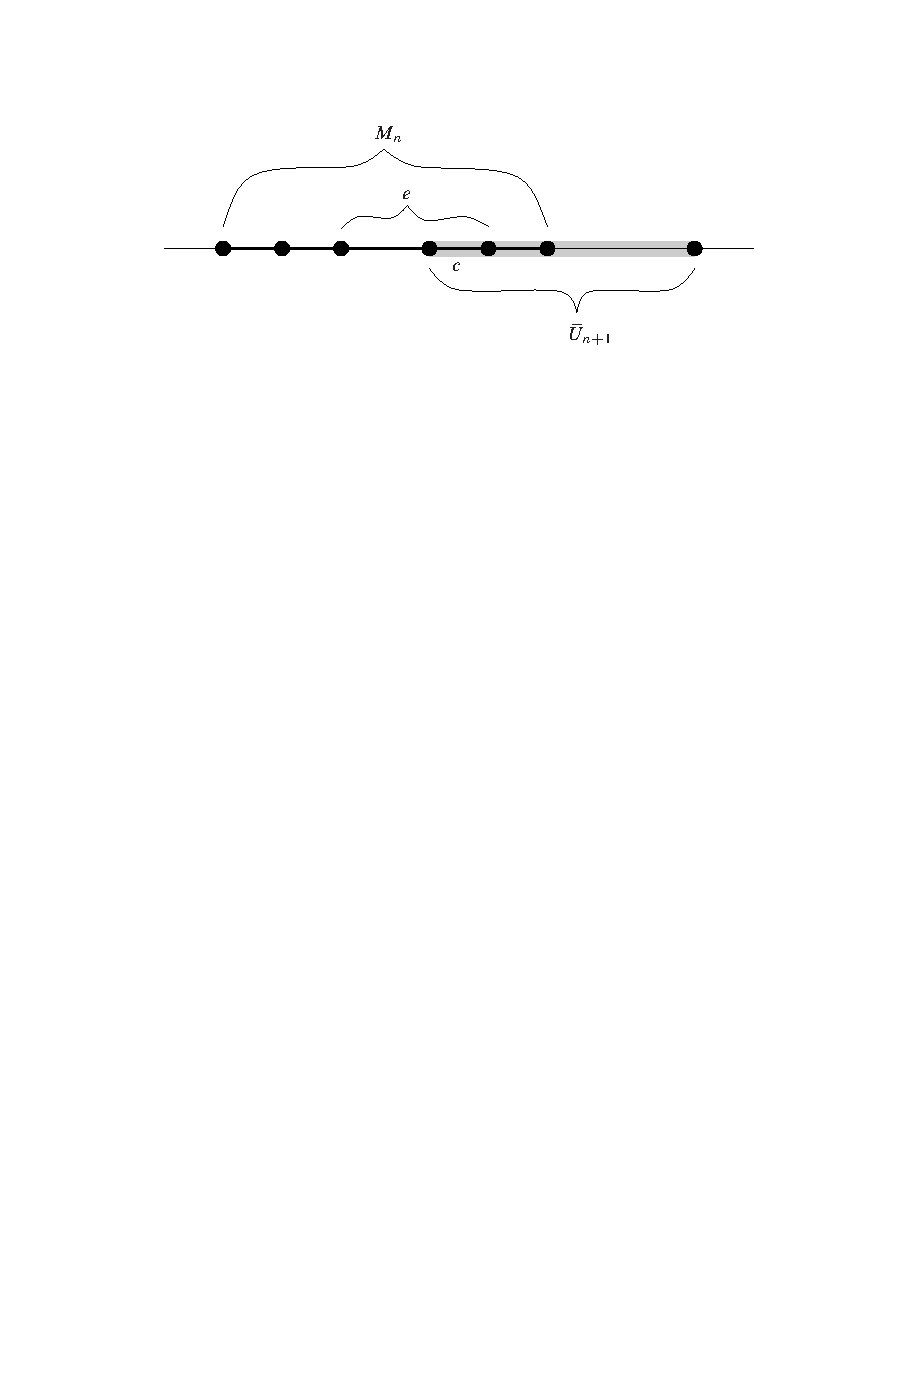
\includegraphics{1-maniCW.pdf}
\caption{Proof that $c\sub e$}
\end{figure}
Now let $\mathcal{E}_{n+1}$ be the union of $\mathcal{E}_n$ together with the collection of all the cells in $\mathcal{C}$ that are not contained in any of the cells of $\mathcal{E}_n$. Then $M_{n+1}$ is the disjoint union of the cells in $\mathcal{E}_{n+1}$ by construction. The boundary of each new $1$-cell is a pair of $0$-cells in $\mathcal{E}_{n+1}$ (either ones that were already in $\mathcal{E}_n$ or new ones that were added). Therefore, $\mathcal{E}_{n+1}$ is a finite regular cell decomposition of $M_{n+1}$. Also, $M_n\sub M_{n+1}$ is a subcomplex because it is the union of the cells in $\mathcal{E}_n$, and contains the closures of all its cells because it is compact. Thus the induction is complete.\par
Let $\mathcal{E}=\bigcup_n\mathcal{E}_n$. The cells in $\mathcal{E}$ are pairwise disjoint (because any two cells lie in $\mathcal{E}_n$ for some $n$), and their union is $M$. If $x$ is any point of $M$, there is some $n$ such that $x\in U_n\sub M_n$. Our construction ensures that all the cells of $\mathcal{E}\setminus\mathcal{E}_n$ are disjoint from $M_n$, and thus $U_n$ is a neighborhood of $x$ that intersects no cells of $\mathcal{E}$ except for those in the finite subcomplex  $\mathcal{E}_n$. Therefore, $\mathcal{E}$ is locally finite. Both conditions (C) and (W) follow from local finiteness (Proposition~\ref{CW locally finite cell}), so this is the required regular CW decomposition.
\end{proof}
\begin{lemma}\label{one mani 0-cell 1-cell}
Suppose $M$ is a $1$-manifold endowed with a regular CW decomposition. Then the boundary of every $1$-cell of $M$ consists of exactly two $0$-cells, and
every $0$-cell of $M$ is a boundary point of exactly two $1$-cells.
\end{lemma}
\begin{proof}
By Proposition~\ref{CW dim mani dim}, the dimension of $M$ as a CW complex is $1$.
If $e$ is any $1$-cell of $M$, then $e$ is an open subset of $M$ by Proposition~\ref{CW n-dim n-cell is open}. By definition of a regular CW decomposition, there is a homeomorphism from $[0,1]$ to $\widebar{e}$ taking $(0,1)$ to $e$, so $\partial e=\widebar{e}\setminus e$ consists of two points contained in the $0$-skeleton. This proves the first claim.\par
To prove the second, suppose  $v$ is a $0$-cell of $M$, and let $e_1,\cdots,e_n$ be the (finitely many) $1$-cells that have $v$ as a boundary point. Define
\begin{equation*}
Y_v=\{v\}\cup e_1\cup\cdots\cup e_n
\end{equation*}
We show that $Y_v$ is a neighborhood of $v$ by showing that its intersection with the closure of each cell is open. The intersection of $Y_v$ with $\widebar{v}=v$ is $v$ itself, and the intersection of $Y_v$ with each $\widebar{e}_i$ is $\widebar{e}_i$ minus a boundary point, hence open in $\widebar{e}_i$. For any other cell $e$, $Y_v\cap\widebar{e}=\emp$. It follows that $Y_v$ is open in $M$. This implies in particular that $Y_v$ is itself a $1$-manifold.\par
If $v$ is not a boundary point of any $1$-cell, then $Y_v=\{v\}$, so $v$ is an isolated point of $M$, contradicting the fact that $M$ is a $1$-manifold ($v$ is not a $1$-manifold). If $v$ is a boundary point of only one $1$-cell, then $Y_v$ is homeomorphic to $[0,1)$, which is a contradiction because $[0,1)$ is not a $1$-manifold. On the other hand, suppose $v$ is a boundary point of the $1$-cells $e_1,\cdots,e_k$ for $k\geq3$. Because $Y_v$ is a $1$-manifold, $v$
has a neighborhood $W\sub Yv$ that is homeomorphic to $\R$, and therefore $W\setminus\{v\}$ has exactly two components. But $W\setminus\{v\}$ is the union of the disjoint open subsets $W\cap e_1,\cdots,W\cap e_k$. Each of these is nonempty, because $W\cap\widebar{e}_i$ is nonempty and open in $\widebar{e}_i$. Therefore, $W\setminus\{v\}$ has at least $k$ components, which is a contradiction.\par
The only other possibility is that $v$ is a boundary point of exactly two $1$-cells.
\end{proof}
Now we are ready for the main theorem of this section.
\begin{theorem}[\textbf{Classification of $\bm{1}$-Manifolds}]\label{class one mani}
Every nonempty connected $1$-manifold is homeomorphic to $S^1$ if it is compact, and $\R$ if it is not.
\end{theorem}
\begin{proof}
Let $M$ be a nonempty connected $1$-manifold. By the previous results, we may assume that $M$ is endowed with a $1$-dimensional regular CW decomposition. Thus $M$ is a graph, in which every edge ($1$-cell) has exactly two vertices ($0$-cells)
as boundary points and every vertex is a boundary point of exactly two edges.\par
We define doubly infinite sequences $(v_j)_{j\in\Z}$ of vertices and $(e_j)_{j\in\Z}$ of edges, such that for each $j$ , $v_{j-1}$ and $v_j$ are the two distinct boundary points of $e_j$, and $e_j$, $e_{j+1}$ are the two distinct edges that share the boundary point $v_j$. Choose a vertex $v_0$ arbitrarily, and let $e_1$ be one of the edges that have $v_0$ as a boundary point. Then $e_1$ has exactly one other boundary point distinct from $v_0$; call it $v_1$.\par
Assuming by induction that we have defined $v_0,\cdots,v_n$ and $e_1,\cdots,e_n$ satisfying the given conditions, we let $e_{n+1}$ be the unique edge different from $e_n$ that shares the vertex $v_n$, and let $v_{n+1}$ be the boundary point of $e_{n+1}$ different from $v_n$. Working similarly in the other direction, let $e_0$ be the unique edge other than $e_1$ that has $v_0$ as a boundary point, let $v_{-1}$ be the unique vertex of $e_0$ other than $v_0$, and then continue by induction to define $v_{-n}$ and $e_{-n}$ for $n\in\N$.\par
For each $n\in\Z$, let $F_n:[n-1,n]\to\widebar{e}_n$ be a homeomorphism that takes $n-1$ to $v_{n-1}$ and $n$ to $v_n$, and define a map $F:\R\to M$ by setting $F(x)=F_n(x)$ when $x\in[n-1,n]$, $n\in\Z$. By the pasting lemma, $F$ is continuous.\par
We now distinguish two cases.\par
\begin{itemize}
\item \textit{The vertices $v_n$ are all distinct}. In this case, $\widebar{e}_m\cap\widebar{e}_n\neq\emp$ if and only if $m=n-1$, $n$ or $n+1$, and it follows easily that $F$ is injective. If $B\sub M$ is compact, then $B$ is contained in a finite subcomplex by Theorem~\ref{CW subset compact iff}. Therefore, $F^{-1}(B)$ is a closed subset of $[-C,C]$ for some constant $C$, so it is compact. Thus $F$ is a proper map.\par
The image of $F$ is closed because $F$ is a proper map (Theorem~\ref{prop map closed}). To see that it is also open, for each vertex $v_n$, let $Y_n=\{v_n\}\cup e_n\cup e_{n+1}$; then the same argument as in the proof of Lemma~\ref{one mani 0-cell 1-cell} shows that $Y_n$ is an open subset of $M$. Since $F((n-1,n+1))=Y_n$, the image of $F$ is the open subset $\bigcup_nY_n$. Because $M$ is connected, $F$ is surjective, and thus by Corollary~\ref{prop map lem} it is a homeomorphism. This proves that $M\approx\R$ in this case.
\item $v_j=v_{j+k}$ for some $j$ and some $k>0$. Choose $j$ and $k$ so that $k$ is the smallest such integer possible. By our construction of the sequence $(v_j)$, it follows that $k\geq2$, and the vertices $v_{j+1},\cdots,v_{j+k}$ are all distinct. In addition, the edges $e_{j+1},\cdots,e_{j+k}$ are also distinct, because if any two were equal, there would be a vertex $v_{j'}=v_{j'+k'}$ with $0<k'<k$, contradicting the minimality of $k$.\par
Let $\widehat{F}$ be the restriction of $F$ to the compact interval $[j,j+k]\sub\R$. Then the image of $\widehat{F}$ is closed by the closed map lemma, and it is open by essentially the same argument as in the preceding paragraph, noting that $v_j=v_{j+k}$ and $Y_j=\widehat{F}\big([j,j+1)\cup(j+k-1,j+k]\big)$. It follows that $\widehat{F}$ is surjective, so it is a quotient map. By our choice of $j$ and $k$, the only nontrivial identification made by $\widehat{F}$ is $\widehat{F}(j)=\widehat{F}(j+k)$. The quotient map $G:[j,j+k]\to S^1$ defined by $G(t)=e^{2\pi it/k}$ makes exactly the same identification as $\widehat{F}$, so it follows from the uniqueness of quotient spaces that $M\approx S^1$.
\end{itemize}
\end{proof}
\begin{corollary}[\textbf{Classification of $\bm{1}$-Manifolds with Boundary}]\label{class one mani boundary}
A connected $1$-manifold with nonempty boundary is homeomorphic to $[0,1]$ if it is compact, and to $[0,\infty)$ if not.
\end{corollary}
\begin{proof}
Let $M$ be such a manifold with boundary, and let $D(M)$ be the double of $M$ (Example~\ref{double mani}). Then $D(M)$ is a connected $1$-manifold without boundary, so it is homeomorphic to either $S^1$ or $\R$, and $M$ is homeomorphic
to a proper connected subspace of $D(M)$. If $D(M)\approx S^1$, we can choose a point $p\in D(M)\setminus M$ and obtain an embedding $M\hookrightarrow D(M)\setminus\{p\}\approx\R$, so in either case, $M$ is homeomorphic to a connected subset of $\R$ containing more than one point, which is therefore an interval. Since $M$ has a nonempty boundary, the interval must have at least one endpoint. If it is a closed bounded interval, it is a closed $1$-cell and thus homeomorphic to $[0,1]$; otherwise it is one of the types $[a,b)$, $[a,\infty)$, $(a,b]$ or $(-\infty,b]$, all of which are homeomorphic to $[0,\infty)$.
\end{proof}
\section{Exercise}
\begin{exercise}\label{CW minus n-cell}
Suppose $X$ is an $n$-dimensional CW complex with $n\geq 1$, and $e$ is any $n$-cell of $X$. Show that $X\setminus e$ is a subcomplex, and $X$ is homeomorphic to an adjunction space obtained from $X\setminus e$ by attaching a single $n$-cell.
\end{exercise}
\begin{exercise}\label{extension maps on boundary of cell}
Suppose $D$ and $D'$ are closed cells (not necessarily of the same dimension).
\begin{itemize}
\item[$(a)$] Show that every continuous map $f:\partial D\to\partial D'$ extends to a continuous map $F:D\to D'$, with $F(\Int D)\sub\Int D'$.
\item[$(b)$] Given points $p\in\Int D$ and $p'\in\Int D'$, show that $F$ can be chosen to
take $p$ to $p'$.
\item[$(c)$] Show that if $f$ is a homeomorphism, then $F$ can also be chosen to be a homeomorphism.
\end{itemize}
\end{exercise}
\begin{proof}
Use the proof of Proposition~\ref{CW compact convex is n-cell}.
\end{proof}
\begin{exercise}\label{closed cell exercise}
Suppose $D$ is a closed $n$-cell, $n\geq1$.
\begin{itemize}
\item[$(a)$] Given any point $p\in\Int D$, show that there is a continuous function
$F:D\to[0,1]$ such that $F^{-1}(1)=\partial D$ and $F^{-1}(0)=\{p\}$.
\item[$(b)$] Given a continuous function $f:\partial D\to[0,1]$, show that $f$ extends to a continuous function $F:D\to[0,1]$ that is strictly positive in $\Int D$.
\end{itemize}
\end{exercise}
\begin{proof}
Assume $D=\B^2$, we can choose
\[F(x)=|x|f\Big(\dfrac{x}{|x|}\Big)+\dfrac{1-|x|}{2}\]
with $F(0):=1/2$.
\end{proof}
\begin{exercise}\label{mani is homogeneous}
Recall that a topological space $X$ is said to be \textbf{topologically homogeneous} if for every pair of points in $X$ there is a homeomorphism of $X$ taking one point to the other. This exercise shows that every connected manifold is
topologically homogeneous.
\begin{itemize}
\item[$(a)$] Given any two points $p,q\in\B^n$, show that there is a homeomorphism $\varphi:\widebar{\B}^n\to\widebar{\B}^n$ such that $\varphi(p)=q$ and $\varphi|_{\partial\B^n}=id_{\partial\B^n}$.
\item[$(b)$] For any topological manifold $X$, show that every point of $X$ has a
neighborhood $U$ with the property that for any $p,q\in U$, there is a homeomorphism from $X$ to itself taking $p$ to $q$.
\item[$(c)$] Show that every connected topological manifold is topologically homogeneous.
\end{itemize}
\end{exercise}
\begin{proof}
For a point $x\in\widebar{\B}^n$, denote the intersection of the line starting from $p$ through $x$ with $\partial\B^n$ by $\psi(x)$. It is clear that $\psi(x)=x$ if $x\in\partial\B^n$ and that $\psi$ is continuous. Now define $\varphi$ to be
\[\varphi(x)=q+\dfrac{|p-x|}{|p-\psi(x)|}(\psi(x)-q)\]
and $\varphi(p)=q$.\par
Now choose a regular coordinate ball $U$ to cover $x\in X$, and for this regular ball we can define the homeomorphism to be $\varphi$ in $U$, and identity outside $U$, where $\varphi$ is defined through the homeomorphism $U\to\B^n$. Since $\varphi$ restrics to identity on the boundary of $U$, this function is continuous.
Finnaly, Since $X$ is connected, it is also path connected. Use a path to extract a finite set of points $p,x_1,\cdots,x_n,q$ where adjacent points lie in the same neighborhood satisfying the property of $(b)$. Now define the homeomorphism to be the composition sending $p\to x_1$, $x_1\to x_2$, $\cdots$, $x_n\to q$.
\end{proof}
\begin{exercise}
Generalize the argument of Exercise~\ref{mani is homogeneous} to show that if $M$ is a connected topological manifold and $(p_1,\cdots,p_k)$ and $(q_1,\cdots,q_k)$ are two ordered $k$ tuples of distinct points in $M$, then there is a homeomorphism $F:M\to M$ such that $F(p_i)=q_i$ for $i=1,\cdots,k$.
\end{exercise}
\begin{proof}
By suitble choice of paths, we can move a point with the other points fixed. For $\varphi_m$ such that $\varphi(p_i)=q_i$, $i\leq m$. Choose a path and neighborhood not containing $q_i$ for $i\leq m$. And use this path to move $\varphi_m(p_{m+1})$ to $q_{m+1}$. Composing with $\varphi_i$ gives a homeomorphism $\varphi_{m+1}$ such that $\varphi_{m+1}(p_i)=q_i$ for $i\leq m+1$.
\end{proof}
\begin{exercise}
Suppose $X$ is a topological space and $\{X_\alpha\}$ is a family of subspaces whose union is $X$. Show that the topology of $X$ is coherent with the subspaces $\{X_\alpha\}$ if and only if it is the finest topology on $X$ for which all of the inclusion maps $i_\alpha:X_\alpha\hookrightarrow X$ are continuous.
\end{exercise}
\begin{proof}
Assume the topology on $X$ is coherent with $\{X_\alpha\}$, denote its topology by $\mathcal{T}$. Assume that there is another topology $\mathcal{T}'$ on $X$ such that the inclusions are continuous. Then for every $U\in\mathcal{T}'$ we have $U\cap X_\alpha$ is open in $X_\alpha$ by the simple observation
\[i_\alpha^{-1}(U)=U\cap X_\alpha.\]
Then $U\in\mathcal{T}$ by definition of coherence. This gives $\mathcal{T}'\sub\mathcal{T}$, which means $\mathcal{T}$ is the finest.\par
Now assume that the topology $\mathcal{T}$ is the finest, for any subset $U$ such that $U\cap X_\alpha$ is open in $X_\alpha$, define a topology on $X$ by $\mathcal{T}'=\{\emp,U,X\}$. Then with $\mathcal{T}'$, the inclusion map is continuous, so we have $\mathcal{T}'\sub\mathcal{T}$, which means $U$ is open in $X$. Thus $\mathcal{T}$ is coherent with $\{X_\alpha\}$.
\end{proof}
\begin{exercise}\label{space coherent topology eg}
Suppose $X$ is a topological space. Show that the topology of $X$ is coherent
with each of the following collections of subspaces of $X$:
\begin{itemize}
\item Any open cover of $X$.
\item Any locally finite closed cover of $X$.
\end{itemize}
\end{exercise}
\begin{proof}
For the first point, just observe that
\[U=\bigcup_\alpha(U\cap X_\alpha)\]
so we prove for open sets.\par
For the second point, this union becomes a finite union. So prove the closed set.
\end{proof}
\begin{exercise}
Here is another generalization of the pasting lemma. Suppose $X$ is a topological space whose topology is coherent with a collection $\{X_\alpha\}$ of subspaces of $X$, and for each $X_\alpha$ we are given a continuous map $f_\alpha:X_\alpha\to Y$ such that $f_\alpha|_{X_\alpha\cap X_\beta}=f_\beta|_{X_\alpha\cap X_\beta}$ for all $\alpha$ and $\beta$. Show that there exists a unique continuous map $f:X\to Y$ whose restriction to each $X_\alpha$ is $f_\alpha$.
\end{exercise}
\begin{proof}
Define $f$ in the natural way. For $U\sub Y$ open, $f_\alpha^{-1}(U)=f^{-1}(U)\cap X_\alpha$ is open in $X_\alpha$ since $f_\alpha$ is continuous. And hence open in $X$ by the coherence.
\end{proof}
\begin{exercise}
Show that every CW complex is locally path-connected. Show that every CW complex is compactly generated.
\end{exercise}
\begin{proof}
The first in clear. The second comes from the collection $\mathcal{E}=\{\widebar{e}:e\in X\}$: if $U\cap K$ is closed for any compact subset $K$, then in particular $U\cap\widebar{e}$ is closed. And from (W) we know that $U$ is closed in $X$.
\end{proof}
\begin{exercise}
Let $\P^n$ be $n$-dimensional projective space. The usual inclusion $\R^{k+1}\sub\R^{n+1}$ for $k<n$ allows us to consider $\P^k$ as a subspace of $\P^n$. Show that $\P^n$ has a CW decomposition with one cell in each dimension $0,\cdots,n$, such that the $k$-skeleton is $\P^k$ for $0<k<n$.
\end{exercise}
\begin{proof}
Prove by induction. The result holds for $n=1$ clearly since $\P^1\approx S^1$. Assume the result for $n-1$, define a map $\widebar{\B}^n\to\R^{n+1}\setminus\{0\}$ by
\[F(x_1,\cdots,x_{n})=\big(x_1,\cdots,x_n,\sqrt{1-|x|^2}\big)\]
this maps $\B^n$ to the upper semisphere of $S^n$, with $\partial\B^n$ to $S^{n-1}\times\{0\}$ in $\R^{n+1}$. Assume $q$ is the quotient map $\R^{n+1}\to\P^n$, then $q\circ F:\widebar{\B}^n\to\P^n$ serves as a characteristic map for an $n$-cell.
\end{proof}
\begin{exercise}
Let $\CP^n$ be $n$-dimensional complex projective space, show that $\CP^n$ has a
CW decomposition with one cell in each even dimension $0,2,\cdots,2n$, such that the $2k$-skeleton is $\CP^k$ for $0<k<n$.
\end{exercise}
\begin{proof}
First we show that $\CP^1\approx S^2$. In fact, any $(z_1,z_2)\in\C^2$ with $z_2\neq 0$ can be written into $(z_1/z_2,1)$. And this corresponds the complex plane. For the 
points $(z_1,0)$, they corresponds one point $(1,0)$ in $\CP^1$. So $\CP^1\approx\C\cup\{(1,0)\}\approx S^2$. As we know, $S^2$ has a CW decomposition $\B^0\cup\B^2$. 
So the cliam is valid for $n=1$.\par
With the simple observation $\C\approx\B^2$, we can prove tha claim by induction. The map $\widebar{\B}^{2n}\to\C^{n+1}$ is defined by
\[F(x_!,\cdots,x_n)=(x_1+ix_2,\cdots,x_{2n-1}+ix_{2n},\sqrt{1-|x|^2})\]
\end{proof}
\begin{exercise}
Show that every nonempty compact convex subset $D\sub\R^n$ is a closed cell of
some dimension.
\end{exercise}
\begin{exercise}
Show that an abstract simplicial complex is the vertex scheme of a Euclidean
simplicial complex if and only if it is finite-dimensional, locally finite, and
countable.
\end{exercise}
\begin{exercise}
Suppose $\sigma=[v_0,\cdots,v_k]$ is a simplex in $\R^n$ and $w\in\R^n$. If $\{w,v_0,\cdots,v_k\}$ is an affinely independent set, we say that $w$ is affinely independent of $\sigma$. In this case, the simplex $[w,v_0,\cdots,v_k]$ is denoted by $w\ast\sigma$ and is called the \textbf{cone on $\bm{\sigma}$}. More generally, suppose $K$ is a finite Euclidean simplicial complex and $w$ is a point in $\R^n$ that is affinely independent of every simplex in $K$. Define the cone on $K$ to be the following collection of simplices in $\R^n$:
\[w\ast K:=K\cup\{[w]\}\cup\{w\ast\sigma:\sigma\in K\}\]
Show that $w\ast K$ is a Euclidean simplicial complex whose polyhedron is
homeomorphic to the cone on $|K|$. (prove for the vertex scheme)
\end{exercise}
\begin{exercise}
Let $X$ be a regular CW complex.
\begin{itemize}
\item Let $\mathcal{E}$ be the set of (open) cells of $X$, and let $\mathcal{K}$ be the collection of all nonempty finite subsets $\{e_0,\cdots,e_k\}\sub\mathcal{E}$ with the property that the dimensions of $e_0,\cdots,e_k$ are all distinct, and (after reordering if necessary) $e_{i-1}\sub\partial e_i$ for each $i=1,\cdots,k$. Show that $K$ is an abstract
simplicial complex. (if $e_{i-1}\sub\partial e_i$, then $e_i\sub\partial e_k$ for all $i<k$.)
\item Suppose $K$ is a Euclidean simplicial complex whose vertex scheme is
isomorphic to $\mathcal{K}$. Show that $X$ is homeomorphic to $|K|$ via a homeomorphism that sends the closure of each cell of $X$ onto the polyhedron
of a subcomplex of $K$.
\item Show that every finite-dimensional, locally finite, countable, and regular
CW complex is triangulable.
\end{itemize}
\end{exercise}
\begin{proof}
Define by induction. For $n=0$, map the $0$ cells to the corresponding vertices. Assume the map is defined for $X_{n-1}$. For $e^n$ a $n$-cell, let $S=\{e^{n-1}_1,\cdots,e^{n-1}_k\}$ be the set of $n-1$-cells that is contained in $\partial e^n$. We map $e_n$ to the cone of the image of $\{e^{n-1}_1,\cdots,e^{n-1}_k\}$. This gives the map $X_n\to |K|$.
\end{proof}